% Formatvorlage f\"{u}r das Seminar "Robotik und Prozessinformatik"
%
% Technische Universitaet Braunschweig
% Institut fuer Robotik und Prozessinformatik
% Muehlenpfordtstrasse 23
% D-38106 Braunschweig
% GERMANY
%
% http://www.cs.tu-bs.de/rob
%

%
\documentclass[ifn,english,masterarbeit,pdf,cd]{report}
\usepackage{a4}
\usepackage{doku}
\usepackage{german}
\usepackage{longtable}
%\usepackage[draft]{graphicx}
\usepackage{graphicx}
\usepackage{graphics}
\usepackage{bbm}
\usepackage[dvips]{epsfig}
\usepackage{ngerman}
\usepackage{nomencl}
\usepackage{amssymb}
\usepackage{indentfirst}
\usepackage{amsmath}
\usepackage{listings}
\usepackage{color}
\usepackage{url}
\usepackage{caption}
%\captionsetup{margin=10pt,format=hang,justification=justified}
\captionsetup{format=hang}
\usepackage{subfigure}
\usepackage{float}
\usepackage[section]{placeins}
%\usepackage{tocloft}
\usepackage{caption}
\RequirePackage[colorlinks=true,linkcolor=black,citecolor=black,anchorcolor=black,urlcolor=black,hyperindex,plainpages=true,pdfborder = 0 0 0]{hyperref}
%\usepackage{hyperref}
\usepackage{fancyhdr}
\usepackage{titlesec}
\usepackage{titletoc}

\usepackage{tikz}
\usepackage{tikzscale}
\usepackage{pgfplots}
\usepgfplotslibrary{units}
%\usepackage{tocloft}
 
\renewcommand{\headrulewidth}{0.5pt}
%\renewcommand{\footrulewidth}{0.5pt}
%\renewcommand{cmd}{def}
\fancyhf{} 
\fancyhead[R]{\thepage}
\fancyhead[L]{\leftmark} 

\captionsetup{font={large}}

\definecolor{dkgreen}{rgb}{0,0.6,0}
\definecolor{gray}{rgb}{0.5,0.5,0.5}
\definecolor{mauve}{rgb}{0.58,0,0.82}

\lstset{ %
	language=Octave,                % the language of the code
	basicstyle=\normalsize,           % the size of the fonts that are used for the code
%	numbers=left,                   % where to put the line-numbers
%	numberstyle=\tiny\color{gray},  % the style that is used for the line-numbers
	stepnumber=2,                   % the step between two line-numbers. If it's 1, each line 
	% will be numbered
%	numbersep=5pt,                  % how far the line-numbers are from the code
	backgroundcolor=\color{white},      % choose the background color. You must add \usepackage{color}
	showspaces=false,               % show spaces adding particular underscores
	showstringspaces=false,         % underline spaces within strings
	showtabs=false,                 % show tabs within strings adding particular underscores
	frame=single,                   % adds a frame around the code
	rulecolor=\color{black},        % if not set, the frame-color may be changed on line-breaks within not-black text (e.g. commens (green here))
	tabsize=2,                      % sets default tabsize to 2 spaces
	captionpos=b,                   % sets the caption-position to bottom
	breaklines=true,                % sets automatic line breaking
	breakatwhitespace=false,        % sets if automatic breaks should only happen at whitespace
	title=\lstname,                   % show the filename of files included with \lstinputlisting;
	% also try caption instead of title
	keywordstyle=\color{blue},          % keyword style
	commentstyle=\color{dkgreen},       % comment style
	stringstyle=\color{mauve},         % string literal style
	escapeinside={\%*}{*)},            % if you want to add LaTeX within your code
	morekeywords={*,...},              % if you want to add more keywords to the set
%	keepspaces=true,
}

% #######################################################################
% latin alphabet: small letters
\newcommand{\length}{a}
% b
\newcommand{\coefficient}{c}
\newcommand{\offset}{d}
\newcommand{\error}{\boldsymbol{e}}
\newcommand{\force}{\boldsymbol{f}}
\newcommand{\gravity}{\boldsymbol{g}}
\newcommand{\contact}{\boldsymbol{h}}
\newcommand{\iteration}{i}
% j
\newcommand{\fkine}{k}
\newcommand{\load}{\boldsymbol{l}}
\newcommand{\work}{m}
\newcommand{\joints}{n}
% o
\newcommand{\position}{\boldsymbol{p}}

\newcommand{\joint}{\boldsymbol{q}}
\newcommand{\jv}{\boldsymbol{\dot{q}}}
\newcommand{\ja}{\boldsymbol{\ddot{q}}}
\newcommand{\arbi}{q_{a}}
% r
\newcommand{\generation}{s}
\newcommand{\twist}{\boldsymbol{t}}
\newcommand{\direction}{\boldsymbol{u}}
\newcommand{\volume}{v}
\newcommand{\manipulability}{w}
\newcommand{\pose}{\boldsymbol{x}}
\newcommand{\posea}{\boldsymbol{\dot{x}}}
\newcommand{\posev}{\boldsymbol{\ddot{x}}}
% y
% z


% latin alphabet: capital letters as scalars


% latin alphabet: capital letters as matrices
\newcommand{\SVDA}{\boldsymbol{A}}
\newcommand{\selection}{\boldsymbol{B}}
\newcommand{\basef}{\boldsymbol{B}}
\newcommand{\centrifugal}{\boldsymbol{C}}
\newcommand{\tip}{C}
\newcommand{\mass}{\boldsymbol{D}}
\newcommand{\ee}{\boldsymbol{E}}
\newcommand{\objectf}{\boldsymbol{F}}
\newcommand{\grasp}{\boldsymbol{G}}
\newcommand{\scalar}{\boldsymbol{H}}
% I
\newcommand{\Jacobian}{\boldsymbol{J}}
\newcommand{\gain}{\boldsymbol{K}}
\newcommand{\scaling}{\boldsymbol{L}}
\newcommand{\inertia}{\boldsymbol{M}}
\newcommand{\nullspace}{\boldsymbol{N}}
\newcommand{\object}{O}
\newcommand{\positive}{\boldsymbol{P}}
\newcommand{\weighted}{\boldsymbol{Q}}
\newcommand{\quaternion}{Q}
\newcommand{\rotation}{\boldsymbol{R}}
\newcommand{\skewm}{\boldsymbol{S}}
\newcommand{\base}{T}
\newcommand{\SVDU}{\boldsymbol{U}}
\newcommand{\SVDV}{\boldsymbol{V}}
\newcommand{\world}{W}
% X
% Y
% Z


% for bold Greek letters, use \boldsymbol instead of \mathbf
% Greek alphabet: small letters
\newcommand{\orientation}{\boldsymbol\phi}
\newcommand{\angular}{\boldsymbol{\omega}}
\newcommand{\singular}{\sigma}
\newcommand{\torque}{\boldsymbol\tau}
\newcommand{\storque}{\boldsymbol{\tilde{\tau}}}
\newcommand{\steplength}{\gamma}
\newcommand{\velocity}{\boldsymbol\nu}
\newcommand{\anglex}{\theta}
\newcommand{\anglez}{\alpha}
\newcommand{\real}{\eta}
\newcommand{\kon}{\boldsymbol\epsilon}

% Greek alphabet: capital letters

% special symbols

% #######################################################################
% Titelseite
% #######################################################################
\begin{document}
\large \selectlanguage{english}
\pagenumbering{roman}
\begin{titlepage}
    \setcounter{page}{1}
    \let\footnotesize\small
    \let\footnoterule\relax
    \headsep 1.5cm
    \vskip -2cm
    \begin{center}
    	\rule[1\baselineskip]{\textwidth}{1pt}
    	\LARGE\bf Model of serial production line
    	\vskip 1\baselineskip
    	\rule[1\baselineskip]{\textwidth}{1pt}
    \end{center}   
%    \vskip 0.5cm
    \begin{center}        
               {\Large{Student Thesis\\}\par}
                \vskip 0.25cm
                {\large submitted by\\}
                \vskip 0.25cm
                {\Large Pengfei Zheng\\ \large Matriculation Number: 4729268}
                \vskip 0.8cm
                {\large Institut f\"{u}r Robotik und Prozessinformatik}                       
    \end{center}
%    \vskip 1cm
\linespread{1.5}
\begin{table}[!h]
	\centering	
	\begin{tabular}{rl}
		\large	1. Examiner:& \large Prof. Dr. -Ing. Klaus Dr\"{o}der \\
		\large2. Examiner:& \large Prof. Dr. Jochen Steil \\
		% \large3. Examiner:& \large Dr. -Ing. Franz Dietrich \\
		% \large Supervisor:& \large M. Sc. Niels Dehio \\
	\end{tabular}
\end{table}
% \vskip 0.5cm
    \begin{figure}[!h]
        \begin{center}
%            \epsfig{file = TU-Logo.eps}
            
\includegraphics[width=0.3\linewidth]{carolo.jpg}
        \end{center}
    \end{figure}
  %  \vskip 1cm
  %  \centerline{\LARGE\bf Institut f\"{u}r Robotik und Prozessinformatik}
  %  \vskip 1cm
   % \centerline{\LARGE\bf Prof.~Dr.~J.~Steil}
%\vskip 0.25cm
\centerline{\large\bf Technische Universit\"{a}t Braunschweig}
\vskip 1cm
\centerline{\large\bf 2020.01.01}

\end{titlepage}
%\setcounter{footnote}{0}
%\setcounter{totalnumber}{8}

% #######################################################################
% Eidesstattliche
% #######################################################################
\clearpage
\pagenumbering{roman}
\thispagestyle{fancy}
\lhead{\textsl{Eidesstattliche Erkl\"{a}rung}}
\rhead{\textbf{\thepage}}
\cfoot{}
\chapter*{Eidesstattliche Erkl\"{a}rung}

\noindent Ich erkl\"{a}re, dass ich die vorliegende wissenschaftliche Arbeit selbst\"{a}ndig, sowie ohne unerlaubte fremde Hilfe verfasst und nicht anderweitig f\"{u}r Pr\"{u}fungszwecke vorgelegt habe. Alle verwendeten Quellen und Hilfsmittel wurden angegeben, sowie w\"{o}rtliche und sinngem\"{a}"se Zitate als solche gekennzeichnet.

\vskip 0.75cm
\noindent Braunschweig, den 01.01.2020

\vskip 0.75cm
\noindent Pengfei Zheng
\addcontentsline{toc}{chapter}{Eidesstattliche Erkl\"{a}rung}
% #######################################################################
% Acknowledgement
% #######################################################################
\clearpage
%\thispagestyle{headings}
\thispagestyle{fancy}
\lhead{\textsl{Acknowledgement}}
\rhead{\textbf{\thepage}}
\cfoot{}
% --------------------------------------------------------------------------------------
% Acknowledgement (English)
% --------------------------------------------------------------------------------------
% \clearpage
%\pdfbookmark[0]{Abstract}{abstract}
\chapter*{Acknowledgement}
%%\ihead{Abstract}

I would like to express my special thanks to Prof. Dr. Jochen Steil as well as my supervisor Tianran Wang for professional guidance and valuable support. They helped me in understanding and going deep into my topic in the early stages of the work, and later also gave me many valuable suggestions and inspirations when I was in difficulty. I am really grateful to them.
\addcontentsline{toc}{chapter}{Acknowledgement}

% #######################################################################
% Abstract
% #######################################################################
\clearpage
% \thispagestyle{headings}
\thispagestyle{fancy}
\lhead{\textsl{Abstract}}
\rhead{\textbf{\thepage}}
\cfoot{}
% --------------------------------------------------------------------------------------
% Abstract (English)
% --------------------------------------------------------------------------------------
%\cleardoublepage
%\pdfbookmark[0]{Abstract}{abstract}
\chapter*{Abstract}
%%\ihead{Abstract}
\setlength{\parindent}{2pc}
\noindent In the past few years, due to the global energy crisis and rapid expansion of production requirement improving productivity and reducing energy consumption have received extensively focus. Therefore, manufacturing system which aims to improve operation control efficiency and results in energy sparing, has been widely studied. Steady state analysis of prodution systems has obtained broadly investigated. On the contrary, the trasient performance remained largely unexplored. This research mainly focus on system modeling, transient performance evaluation, and production line parameter optimization. Indeed, transient behavior of production systems has generally practical and theoretical implications. 

The main contribution of this work is to implement the mathematical models in a high-level programming language, python, and make a result analysis. Furthermore, we also designed a experiment to find a optimized buffer size to improve the transient performance of the production lines.


\vskip 0.75cm
\noindent\textbf{Keywords:} Geomatric Machine, Production Lines, mathmaticall model, performance evaluation, transient analysis.
\addcontentsline{toc}{chapter}{Abstract}

% % #######################################################################
% % Inhaltsverzeichnis
% % #######################################################################%
% \clearpage
% %\pagenumbering{roman}

% %\pagestyle{fancy}
% %\fancyfoot[R]{\thepage}
% %\pagestyle{myheadings}
% \thispagestyle{fancy}
% \lhead{\textsl{Contents}}
% \rhead{\textbf{\textbf{iv}} }
% \cfoot{}
% \addtocontents{toc}{\protect\thispagestyle{fancy}}
% \pdfbookmark[0]{Contents}{anchor}
% \tableofcontents

% %\renewcommand{\headrulewidth}{1pt}
% %\setlength{\baselineskip}{3ex}
% %\rhead{45}

% %\renewcommand{\headrulewidth}{0pt}
% %\afterpage{\lhead{new value}}

% \clearpage
% \setcounter{page}{5}
% \thispagestyle{fancy}
% \lhead{\textsl{List of Figures}}
% \rhead{ \textbf{\thepage} }
% \cfoot{}
% \listoffigures
% \addcontentsline{toc}{chapter}{\listfigurename}

% \clearpage
% \setcounter{page}{8}
% \thispagestyle{fancy}
% \lhead{\textsl{List of Tables}}
% \rhead{\textbf{\thepage}}
% \cfoot{}
% \listoftables
% \addcontentsline{toc}{chapter}{\listtablename}
% % #######################################################################
% % Dokument
% % #######################################################################

\cleardoublepage

\chapter{Introduction}
\pagenumbering{arabic}
\setlength{\parindent}{2pc}
\label{intro}
% #######################################################################
\noindent 
Production system has been studied widely during the last 65 years \cite{papadopolous1993queueing}. A production system is an industrial system that describe a procedure to transform from different resources into useful products. In this process, producing units (human operators, industrial robots, cells, etc.) and resource handling devices (shelves, carts, holders, vehicles, etc.) connected with each others so that desired products can be produced. It is a very important part of manufacturing research and application. 

% Extensive research has been invested in develpoing for design, modeling, improvement, analysis and control of production systems (for instance, monographs \cite{buzacott1993stochastic, askin1993modeling, bonomi1987approximate, rao2000performance}). Despite the fact that in practice production systems may take several kinds of physical topologies, serial lines [see Figure \ref{Serial line.}] and assembly systems [see Figure \ref{Assymbly system.}] are the two most basic structures used in different manufacturing environments. In the literature, meanwhile, while serial production lines have been extensively investigated, assembly systems are been paid much less attention. Early research on assembly systems only considered the cases of multi-sequence-single-server, where different types of parts arrive at a single server in oder to be assembled together \cite{harrison1973assembly, bonomi1987approximate}. Inspired by these works, few three-server system with limited sequence capacities have been studied. In these papers, dual servers represent component part production, and other servers represent assembly operations.


\begin{figure*}[!h]
	\centering
	\subfigure[Serial line.]{
		\includegraphics{figures/serial_line.tikz}
		\label{Serial line.}}
	\subfigure[Assymbly system.]{
		\includegraphics{figures/assembly_system.tikz}	
	 	\label{Assymbly system.}}
	\caption{two production system}
	\label{Serial productionline and assembly system.}
\end{figure*}


The steady state behavior of production systems has been deeply studied in the last few years. Although it is often difficult to declare from the partial view that a production system is in steady state, the steady-state analysis approach is effective and accurate enough for manufacturing systems with large production capacity. The large production capacity allows the system to decay instantaneously to a negligible time compared to the global production run-time, and, therefore, allows it to use steady-state methods. Unfortunately, in addition to large-capacity manufacturing, there are a large number of mid- and small-capacity manufacturing systems in practice, which usually operate in a different method. In some these cases, one production line is usually able to produce several end products but can only produce one type of end product, equipment or special product at a time because of process. This usually lead to small- to medium-size production run-based operation based on the customer's order, where a production run contains only a specific amount of particular type of product. Obviously, when the size of the production run is relatively small, the steady-state approaches cannot provide an ideal and accurate analysis of system. In some industries, a production run somtimes means a batch.

Nevertheless, the transient period of the behavior in production system has received much less research attention because of its complexity and the still large numbers of unsolved problems in steady state production systems research. On the other hand, recent research \cite{li2009throughput} has proved that transient analysis has become one of the most important fields in production systems research. 


% \chapter{Model and Performance Measures}
\label{B_Kapitel}
\noindent This chapter mainly focus on the mathmaticall model, the first part introduces the theoretical basis of the mathmaticall mode, and the assumptions to build such mathmaticall model, the second part presents the performance measures of transient properties.

% #######################################################################
\section{Model}
\noindent Before the discussion of the mathmaticall mode, the classic conception of Markov chain should be first introduced as the theoretical basis of stochastic models to describe a process of real world. This made the foundation of for general stochastic simulation methods known such as Markov chain Mente Carlo, which are suitable for simulating sampling from comlex probability distributions, and also able to be applied in Bayesian statistics and artificial intelligence. Besides, for serial production lines with geometric machines and finite buffers, in particular, there are more assumptions to describe and derive such a system.

% #######################################################################
\subsection{Markov chain}
\noindent A Markov chain is a stochastic model basically describing a sequence of random events in which the probability of each event is related only to the state attained in the previous event \cite{gagniuc2017markov}. In time-continuous situation, it is known as Markov process. It is named after the Russian mathematician Andrey Markov. 

Here is a diagram (see Figure \ref{a two state markov process}) representing a two state Markov process, where the states are labelled as A and B respectively. Every number represents the probability of the Markov process transforming from one state to another state with the arrow that indicates the direction. For instance, if the Markov process is now in state B, then the probability it transforms to state A is 0.6, while the probability it remains in state B is 0.4.

\begin{figure}[!h]
	\centering
	\includegraphics[]{a_markov_model.tikz}
	\caption{A two-state Markov process}
	\label{a two state markov process}
\end{figure}

The precise definition of the conception ''Markov chain'' will be given as following. A Markov process is a certain type of stochastic process distiguished by the Markov property \cite{chung1967markov}. A Markov chain is a Markov process with a calculable (namely, finit or denumerably infinite) number of states. The time parameters can be taken as the set of nonnegative integers or the set of nonnegative real numbers, so we have discrete parameter cases or continuous parameter cases. The adjective ''simple'' is sometimes used to qualify the Markov chain, but since we really do not discuss the ''multiple'' chains we should not treat it differently. In addition, we should only discuss the Markov chains which has a '' stationary (or temporally homogeneous) transition probabilities'' so that the qualifying expression in quotes will be understood. In the end, our discussion does not distinguish between a finite or a calculable infinite number of states and therefore we does not do any special treatment for the former case.

In this part we handle the case of a discrete parameter. Here the essential foundations can be summarized as follows.

Suppose we have an abstract set $ \probspace $ , called the probability space, having the generic element $ \genericelement $, called elementary event; a Borel field $\Borelfield $ of subsets of $ \probspace $ , called measurable sets or events, where $\probspace$ is considered as a member; and a probability measure $\probmeasure $ defined on $\Borelfield $. The triple $\parens{\probspace, \Borelfield, \probmeasure} $ is named as a probability triple. A set in $\Borelfield$ of probability zero will be named as a null set; ''almost all $\genericelement$ (a.a.$\genericelement$)'' or ''almost everywhere (a.e.)'' expresses ''all $\genericelement$ except a null set''. The pair $\parens{\Borelfield, \probmeasure} $ will be regarded to be complete in the sense that each subset of a null set is attached to $\Borelfield$ and is a null set. If and only if a Borel subfield of $\Borelfield$ contains all null sets, it is said to be augmented. If a Borel subfield is given, there exists a unique smallest augmented Borel subfield of $\Borelfield$ including the given one. Unless exceptions specified all the following Borel fields will be presumed to be augmented. A (real) random variable is regarded as a single-valued function from a set $\domainod$ in $\Borelfield$ to the closed real line $X = [-\infty,+\infty]$ thus for every real number $c $ the set of $\genericelement$ in $\domainod$ for which $x(\genericelement) \leq c$ is attached to $\Borelfield$. $\domainod$ is named as the domain of definition of $x$ and the set $\domainof$ of $\genericelement$ in $\domainod$ for which $|x(\genericelement)|<\infty$ is named as the domain of finiteness of $x$. If neither domain is specific it will be figured out that $\probmeasure(\domainof)=1$; otherwise stated, the random variable is finite-valued. It comes from the definition that if $A$ is any Borel set in $X$, then the set of $\genericelement $ for which $x(\genericelement)\in A$, to be symbolized as ${\genericelement:x(\genericelement)\in A}$ is attached to $\Borelfield$. The probability of the set comes to be denoted by
\begin{equation}
\probmeasure \{ x(\genericelement)\in A \}.
\end{equation}
Symbols alike to these which will come later should be self-explanatory if we mark that commas or semicolons are served as symbolizing intersection of sets; for instance
\begin{equation}
    \begin{aligned}
    \probmeasure\{x_\nu(\genericelement)\leq c_\nu,1\leq \nu\leq 2\}&=\probmeasure\{x_1(\genericelement)\leq c_1; x_2(\genericelement)\leq c_2\} \\ &= \probmeasure\left\{\cap_{n=1}^2 [x_n(\genericelement)\leq c_n]\right\}.
    \end{aligned}
\end{equation}
Suppose we hold a set $\{x_s, s\in S\}$ of random variables, the Borel field created by them is the smallest augmented Borel field regarding which all the random variables in the set are able to be measured. Special cases are $\Borelfield\{x_s,s\circ t\}$ where $\circ$ is one of the four symbols $<, \leq , >, \geq$.

The function $F$ described by
\begin{equation}
    F(u)=\probmeasure\{x(\genericelement)\leq u\}
\end{equation}
for all real $u$ is named as the distribution function of $x$. We get such that
\begin{equation}
    \lim_{u\to +\infty} F(u) - \lim_{u\to -\infty} F(u) = \probmeasure(\domainof).
\end{equation}
Unless otherwise stated, we will use a distribution function or a probability distribution that of a random variable which is limited with probability one to represent. Thus $\lim_{u\to -\infty} F(u) = 0$, $\lim_{u\to +\infty} F(u) = 1$. A random variable $x$ is discrete if and only if there exists a calculable set $A$ thus $P\{x(\genericelement)\in A\} = 1$. A possible value $c$ of $x$ is just one like $\probmeasure\{x(\genericelement)=c\}>0$. All random variables engaged in the part are discrete. A function $x$ from $\domainod$ in $\Borelfield$ to a calculable set $A$ can be taken as a random variable if and only if the set $\{ \genericelement : x(\genericelement) = c\}$ is attached to $\Borelfield$ for every $c$ in $A$. Actually $A$ could be assigned as any abstract calculable set and we could define an abstract-valued random variable like this.

Suppose $\Lambda_1$ and $\Lambda_2$ are two sets in $\Borelfield$, the conditional probability of $\Lambda_2$ in relation to $\Lambda_1$ is defined By
\begin{equation}
    \probmeasure(\Lambda_2|\Lambda_1) = \frac{\probmeasure(\Lambda_1 \Lambda_2)}{\probmeasure(\Lambda_1)}
\end{equation}
given that $\probmeasure(\Lambda_1)>0$. When $\probmeasure(\Lambda_1)=0$, $\probmeasure(\Lambda_2|\Lambda_1)$ is undefined. For convenience, undefined conditional probabilities will often be seen in following. If one that comes our from them is multiplied by a variable which is equal to 0, the product is considered to be 0. The conditional probability of the set $\{\genericelement :x_3(\genericelement) = c_3\}$ in relation to the set $\cap_{n-1}^2 \{\genericelement : x_n(\genericelement)=c_n\}$ for example is symbolized as
\begin{equation}
    \probmeasure\{x_3(\genericelement)=c_3|x_1(\genericelement)=c_1, x_2(\genericelement)=c_2\}.
\end{equation}

For the random variables $\{x_\nu, 1\leq \nu \leq n\}$, it is not necessarily finite-valued, and is said to be independent in case
\begin{equation}
\probmeasure \left\{\bigcap_{\nu=1}^n [x_\nu(\genericelement)\leq c_\nu]\right\} = \prod_{\nu =1}^n \probmeasure\{x_\nu (\genericelement)\leq c_\nu\}
\end{equation}
for any real finite $c_\nu$, $1\leq \nu \leq n$. It comes out that the same equation remains true if the sets $\{\genericelement :x_\nu (\genericelement)\leq c_\nu\}$ are changed to the more general sets ${\genericelement :x_\nu(\genericelement)\in A_\nu}$ where the $A_\nu$ are Borel sets in $X$. Suppose we habe a sequence $\{x_n,n\geq 1\}$, it is a sequence of independent random variables only if any finite number of them are independent. The denumerable sets $\Lambda_\nu$, $1\leq \nu \leq n$ or $1\leq \nu < \infty$ are independent only if their indicators are, the indicator of a set rendered as the function which on the set end is equal to one zero elsewhere.

The mathmaticall expectation of a random variable $x$ can be give by the abstract Lebesgue-Stieltjes integral
\begin{equation}
    \expectation(x) = \int_{\probspace} x(\genericelement) \probmeasure(d\genericelement).
\end{equation}
In general, we extend this definition to a random variable that supposes that only if the integral existing, one of two values $+\infty$ or $-\infty$ with positive probability is finite or infinite. The conditional expectation of $x$ relative to $\Lambda$, provided $\Lambda \in \Borelfield$, is defined as
\begin{equation}
    \expectation(x|\Lambda) = \int_{\probspace}x(\genericelement) \probmeasure(d\genericelement|\Lambda) = \frac{\int_{\probspace}x(\genericelement) \probmeasure(d\genericelement)}{\probmeasure(\Lambda)}.
\end{equation}
Specially if $x$ is discrete with all its probable quantities in the measurable set $A$ then
\begin{equation}
    \expectation(x|\Lambda)=\frac{1}{\probmeasure} \sum_{i\in A} i\probmeasure\{\Lambda; x(\genericelement)= i\}
\end{equation} 
as long as the series is fully converged.

In this part the letters $n, m, \nu, r ,s ,t $ denote non-negative integers unless otherwise stated.

A discrete parameter stochastic process is described as a sequence of random variables $\{x_n, n\geq 0\}$ defined regarding a probability triple $(\probspace, \Borelfield, \probmeasure)$. If all random variables are discrete, the union $\statespace$ of all probable quantities of all $x_n$ is a countable set named as the minimum state space of the process and every element of $\statespace$ is a state. Therefore, $i\in \statespace$ if and only if there is an $n \geq O$ so as $\probmeasure\{x_n(\genericelement) = i\} >  O$. We take from the language of physics where the term ''state'' indicates that of a  material system whose evolution in time is characterized by our stochastic process model.

A discrete parameter Markov chain can be defined by a sequence of discrete random variables $\{x_n, n\geq O\}$ possessing the under property: for arbitrary $n \geq 2$, $O\geq t_1 < ... < t_n$ and arbitrary $i_1, ... , i_n$ in the state space $\statespace$ we have
\begin{equation}
    \left\{
        \begin{aligned}
       \probmeasure \{x_{t_n}(\genericelement) &= i_n | x_{t_1}(\genericelement) = i_1, ... ,x_{t_{n-1}}(\genericelement) = i_{n-1}\} \\
       &= \probmeasure\{x_{t_n}(\genericelement) = i_n | x_{t_{n-1}}(\genericelement) = i_{n-1}\} .
        \end{aligned}
    \right.
    \label{state space}
\end{equation} 
whenever the left member is defined. The condition \ref{state space} will appear as the Markov property. It is identical to the under apparently weaker condition: for each $n\geq 1$,
\begin{equation}
    \begin{aligned}
        \probmeasure \{x_n(\genericelement) &= i_n| x_0(\genericelement) = i_0,...,x_{n-1}(\genericelement)=i_{n-1}\} \\ &=\probmeasure \{x_n(\genericelement)=i_n|x_{n-1}(\genericelement)=i_{n-1}\}.
    \end{aligned}
\end{equation}
The proof here is neglected. An important consequence comes from condition \ref{state space} is that for arbitrary $n \geq 0$ and $0\leq t_1<...<t_n...<t_{n+m}$; and arbitrary $i_1,...,i_n,...mi_{n+m}$ in $\statespace$ we get
\begin{equation}
    \left\{
        \begin{aligned}
            \ & \probmeasure\{x_{t_\nu}(\genericelement)=i_\nu, n\leq \nu \leq n+m|x_{t_\nu}(\genericelement)=i_\nu, 1\leq \nu \leq n-1\} \\
            =& \probmeasure \{x_{t_\nu}(\genericelement) = i_\nu, n\leq \nu \leq n+m|x_{t_{n-1}}(\genericelement)=i_{n-1}\}.
        \end{aligned}
        \right.
        \label{state space2}
\end{equation}
The proof of \ref{state space2} is carried out by induction on $m$. For $m = 0$, it decreases to \ref{state space}. Supposing that \ref{state space2} is true for a certain quantity of $m$, it comes to use the rules of combining conditional probabilities and \ref{state space},
\begin{equation}
    \begin{aligned}
        \ & \probmeasure\{x_{t_\nu}(\genericelement)=i_\nu, n\leq \nu \leq n+m+1|x_{t_\nu}(\genericelement)=i_\nu, 1\leq \nu \leq n-1\} \\
        =& \probmeasure\{x_{t_\nu}(\genericelement)=i_\nu, n\leq \nu \leq n+m|x_{t_\nu}(\genericelement)=i_\nu, 1\leq \nu \leq n-1\} \times \\
        \times & \probmeasure\{x_{t_{n+m+1}}(\genericelement)=i_{n+m+1}|x_{t_\nu}(\genericelement)=i_\nu, 1\leq \nu \leq n+m\} \\
        =& \probmeasure\{x_{t_\nu}(\genericelement)=i_\nu, n\leq \nu \leq n+m|x_{t_{n-1}}(\genericelement)=i_{n-1}\} \times \\
        \times & \probmeasure\{x_{t_{n+m+1}}(\genericelement)=i_{n+m+1}|x_{t_{n+m}}(\genericelement)=i_{n+m}\} \\
        =& \probmeasure\{x_{t_\nu}(\genericelement)=i_\nu, n\leq \nu \leq n+m|x_{t_{n-1}}(\genericelement)=i_{n-1}\} \times \\
        \times & \probmeasure\{x_{t_{n+m+1}}(\genericelement)=i_{n+m+1}|x_{t_{\nu}}(\genericelement)=i_{\nu}, n - 1\leq \nu \leq n+m\} \\
        =& \probmeasure\{x_{t_\nu}(\genericelement)=i_\nu, n\leq \nu \leq n+m+1|x_{t_{n-1}}(\genericelement)=i_{n-1}\}.
    \end{aligned}
\end{equation} 
Therefore \ref{state space2} is true when $m$ is replaced by $m+1$ and the induction is complete.

It is well know that a result comes from measure theory asserts that for all $m$ the validity of \ref{state space2} indicates that of the more general result: for each $\markovproperty \in \Borelfield \{x_t, t\geq t_n\}$ we get
\begin{equation}
    \probmeasure \{\markovproperty | x_{t_\nu}(\genericelement) = i_\nu, 1\leq \nu \leq n\} = \probmeasure \{\markovproperty | x_{t_n}(\genericelement)= i_n\}.
    \label{markov property}
\end{equation}
In this expression Markov property can be expressed verbally as positing that ''If we know the state of an event at the previous moments, the probability of it is the same as only the last given state''. More vaguely, it can be presented that ''the past state is completely independent from the future state''. Misleading by these description, it is a normal mistake to believe that Equation \ref{markov property} stays true if the conditional events in it are replaced by a more general event, for instance, replacing $i_\nu$ with $A_\nu$, where $A_\nu$ is a subset of $\statespace$. No doubt the resulting equation will generally be wrong. Nevertheless, the under extension of \ref{markov property} is correct and trivial: if $\Lambda \in \Borelfield\{x_t,t\leq t_n\}$
\begin{equation}
    \probmeasure \{\markovproperty | \Lambda ; x_{t_n}(\genericelement)= i \} = \probmeasure\{\markovproperty |x_{t_n}(\genericelement)= i\}.
\end{equation}

% #######################################################################
\subsection{Descriptive Model}
\noindent Consider a production line shown in Figure \ref{serial production line}, in which circles illustrate machines and rectangles illustrate buffers. The system will be defined by the under assumptions.

\begin{figure*}[!ht]
	\centering
	\includegraphics{serial_line.tikz}
	\caption{Serial production line.}
	\label{serial production line}.
\end{figure*}

\begin{itemize}
    \item[1.] The system is composed of $M$ machines, arranged in series, and $M-1$ buffers between each consecutive pair of machines.
    \item[2.] The machines all have the same constant cycle time $\tau$. The time axis is limited in a slot duration $\tau$. Machines start to operate at the beginning of each time slot.
    \item[3.] The model requires the machine to observe geometric reliability: We use $s_i(n) \in \{0 = down, 1 = up\} $ to symbolize the state of machine $m_i$ during time slot $n, i = 1, ..., M$. Then, we can fomulate the transient probabilities as follow:
    \begin{equation}
        \begin{aligned}
            \text{Prob}[s_i(n+1)=0|s_i(n)=1]=&P_i \\
            \text{Prob}[s_i(n+1)=1|s_i(n)=1]=&1-P_i \\
            \text{Prob}[s_i(n+1)=1|s_i(n)=0]=&R_i \\
            \text{Prob}[s_i(n+1)=0|s_i(n)=0]=&1-R_i
        \end{aligned}
        \label{transition probabilities}
    \end{equation}
    where $ P_i $ and $R_i$ are used to denote the breakdown and repair probabilities separately. Each machine has the operation independence from one another.
    \item[4.] Each buffer is described by its capacity (in other words, the maximum number of products the buffer can preserve), $1 \leq N_i < \infty$, $i = 1, ..., M-1$.
    \item[5.] Machine $m_i, i = 2, ..., M$, is in a state of starved condition in one time slot if it is up (i.e. it works properly) and buffer $b_{i-1}$ is empty at the start of this time slot. Machine $m_1$ will be never starved for there will always be raw material.
    \item[6.] Machine $m_i,i = 1,...,M-1$, is in a blocked state in one time slot if it works properly, buffer $b_i$ has $N_i$ parts at the start of this time slot, and machine $m_{i+1}$ is  to take a product in this time slot. Machine $m_M$ will never be blocked.
    \item[7.] If a machine works well and is neither starved or blocked, it is capable to process one product during a time slot (in other words, takes a product from its upstream buffer at the start of this time slot, processes it within the time slot, and puts it into its downstream buffer at the end of the time slot); otherwise, no processing will occur for the machine in this time slot.
    \item[8.] The system works in a total of T time slots.
\end{itemize}

\textsl{Remark 1}: For the assumption 3, the up and downtime of machine $m_i$ are geometric random values. We can calculate its average up- and downtime through $T_{up,i}=1 / P_i$ and $T_{down,i} = 1/ R_i$, separately. Moreover, the machine efficiency, in other words, the probability (ratio of time) that $m_i$ works properly in steady state, can be calculated by $e_i=T_{up,i}/(T_{up,i}+T_{down,i}) = R_i/(R_i + P_i)$.

\textsl{Remark 2}: When the average downtime of the machine is much longer than its cycle time (for instance, in machining, painting, wielding operations)the geometric reliability is generally applicable. Steady state performance of the geometric serial lines has been explored in numerous publications in manufacturing systems literatures \cite{papadopolous1993queueing,buzacott1993stochastic, gershwin1994manufacturing,altiok1997performance} The geometric model also has a successful application in industrial occasions works (i.e. \cite{li2003due, liberopoulos2007performance}).

\textsl{Remark 3}: These previous assumptions indicate that the failures of machines are time-dependent (in other words, in a state of starvation or blockage a machine may still break down). Another kind of failure model as an optional choice, operation-dependent failure (in other words, in the state of starvation or blockage, a machine will not break down), is also covered in the literature. The properties and behavior of systems established by both declarations are very approximate (by \cite{li2006comparisons}). In this work we consider the former one, time-dependent failures.

\textsl{Remark 4}: Assumption 6. indicates the blocked-before-service (BBS) regulation, under which, a machine may be in a starvation and blockage state in the same time slot. Its similitude, the blocked-after-service (BAS) regulation, is also extensively used in production systems research (see \cite{dallery1992manufacturing, papadopoulos1996queueing,li2009throughput}). The analysis of systems established by both regulations are approximate. In fact, either system models under one regulation can be transformed into the another one with the other regulation by changing the buffer size by one unit. In this work we use BBS regulation, because it results in a simpler statement \cite{li2008production}.


\section{Performance Measures}
\label{performance measures}
\noindent In order to conduct strict control of production systems and real-time evaluation, transient performance measures must be introduced. In the framework of geometric serial lines given by assumptions 1-8, the performance measures of interest are:
\begin{itemize}
    \item[$\bullet$] \textsl{Production Rate}, $PR(n) = $ the expected number of finished parts produced by $m_M$ in time slot $n$;
    \item[$\bullet$] \textsl{Consumption Rate}, $CR(n)=$ the expected number of raw parts consumed by $m_1$ in time slot $n$;
    \item[$\bullet$] \textsl{Work-in-process}, $WIP_i(n)=$ the expected number of parts in buffer $b_i$ at the start of time slot $n$, $i=1,...,M-1$;
    \item[$\bullet$] \textsl{Machine Starvation}, $ST_i(n)=$ Prob[$m_i$ is starved by $b_{i-1}$ in time slot $n$], $i=2,...,M$;
    \item[$\bullet$] \textsl{Machine Blockage},$ BL_i(n)=$ Prob[$m_i$ is blocked by $b_i$ in time slot $n$], $ i=1,...,M-1$.
\end{itemize}
In this paper, we take average of numours simulation results to get these performance measures of interest. It should be noted that, in this paper, a simulation procedure uses least $10000$ the production lines to get the mathematical expectations.
% \chapter{Transient Performance of Various Geomatric Machines}
\label{C_Kapitel}
\noindent In this chapter we will use the programming language to implement these mathmatical models from the simple individual machine to multi-machine and attempt to get the transient performance. In the second section, we will try to analysis the difference between this work and another one. 

We choose to use python as the implementation language because python is a interpreted, general-purpose and object-oriented programming language. With its extensive mathmatics library and other third-party library, it is very popular to be used as a scientific scripting language to aid in a numerical data processing and manipulation problem like this.
% #######################################################################
\section{Individual Geomatric Machine}
\noindent Although transient analysis of individual geometric machines with constant parameters has been studied in \cite{meerkov2010transient}, as the basis of all the following models, we still take it as the primary work. Since the performance evaluation method which we try to derive is the foundation of the study in the this paper, we briefly introduce it below.
\begin{figure}[!h]
	\centering
	\includegraphics[]{figures/model_of_one_machine.tikz}
	\caption{State transition diagram of one geometric machine}
	\label{State transition diagram of one geometric machine}
\end{figure}

% simply copy need to reedit

The state transition schema for an individual geometric machine is illustrated in Figure \ref{State transition diagram of one geometric machine}. We use $x_i(n), i \in \{0=down,1=up\}$ to indicate the probability that the machine is in state $i$ during time slot $n$, that is $x_i(n)=Prob[s(n)=i]$. Apparently, the system is described by a two-state ergodic Markov chain and the transformmation of state vector $x(n)=[x_0(n) \quad x_1(n)]^T$ can be described by
\begin{equation}
	x(n+1) = A_1x(n), x_0(n) + x_1(n) =1
\end{equation}
where
\begin{equation} A_1 = \begin{bmatrix} 1-R&P\\R&1-P \end{bmatrix} \end{equation}

% \begin{math}x(n+1)=A_1 x(n)\end{math}
The production rate and consumption rate of an individual machine with the original state both down(0) and up(1) can be calculated as 
\begin{equation} PR(n)=CR(n)=x_1(n)=\begin{bmatrix} 0&1 \end{bmatrix}x(n)=\begin{bmatrix} 0&1 \end{bmatrix}A_1^n
x(0) \end{equation}

the Figure~\ref{Transients of an individual geomatric machine when it is initially down} is the contrast of simulation and calculation of one geometric machine with initial state of down with the parameters of breakdown
probability $P = 0.05$ and repair probability $R = 0.2$.
which are both linear in machine state $x(n)$.

As an illustration, consider a geometric machine with breakdown probability $P=0.05$ and repair probability $R=0.2$. The transients of the system state and the performance measures are given in Figure \ref{Transients of an individual geomatric machine when it is initially down} and \ref{Transients of an individual geomatric machine when it is initially up}, assuming the machine is initially down and up, respectively. As one can see, the initial condition of a machine has strong impact on system transients—which may result in production loss (see Fig. 3) or production gain (see Fig. 4).

\begin{figure*}[!h]
	\centering
	\subfigure[Result of simulation]{
		\includegraphics[width=6.5cm]{figures/individual_s_0.tikz}
		\label{individual simulation down}}
	\subfigure[Result of calculation]{
		\includegraphics[width=6.5cm]{figures/individual_c_0.tikz}	
	 	\label{individual calculation down}}
	\caption{Transients of an individual geomatric machine when it is initially down}
	\label{Transients of an individual geomatric machine when it is initially down}
\end{figure*}

\begin{figure*}[!h]
	\centering
	\subfigure[Result of simulation]{
		\includegraphics[width=6.5cm]{figures/individual_s_1.tikz}
		\label{individual simulation up}}
	\subfigure[Result of calculation]{
		\includegraphics[width=6.5cm]{figures/individual_c_1.tikz}	
	 	\label{individual calculation up}}
	\caption{Transients of an individual geomatric machine when it is initially up}
	\label{Transients of an individual geomatric machine when it is initially up}
\end{figure*}

In the python code, we use the object-oriented features to help build the model. We seperate the codes into two parts. The first part is a class file called Individual. A \pythoninline{class Individual} represents a geomatirc machine that runs in a two-state Markov chain. It holds the parameters, which are transformed from another file, and calculates once a time slot till the end of the time control parameter \pythoninline{n} changes to zero.
\pythonexternal{pycodes/individual/individual.py}
Another file, which is used to call the \pythoninline{class Individual}, are also attached as following. The main purpose of this file is to calculate the the average values of all the evaluation performance in order to get the mathmatical expectation. The final daten are collected in the file called \pythoninline{result.txt}.
\pythonexternal{pycodes/individual/simu1.py}

\section{Transient Performance of Two-Machine Geometric Lines}
\noindent Consider a two-machine geometric line defined by assumptions 1-8. illustrated in Figure \ref{State transition diagram of two geometric machine with buffer}. It is easy to show that the system is characterized by an ergodic Markov chain. In addition to machine state $si(n)$, let $h(n)$ denote the number of parts in the buffer at the beginning of time slot $n$. Then, the state of the Markov chain is defined by a triple $(h(n),s_1(n),s_2(n))$, where $h(n)\in {0,1,...,N}$ and $s_1(n),s_2(n) \in {0,1}$. Clearly, the system has a total of $4(N+1)$ states. To calculate the transition probabilities among these states, we arrange the states in the following manner: Let $r(h,s1,s2)$ denote the state number of the Markov chain state $(h,s_1,s_2)$, $h\in {0,1,...,N}, s_1,s_2\in {0,1}$. defined
\begin{equation}
	r(h,s_1,s_2) = 4h + 2s_1 +s_2 +1 .
	\label{definition of r}
\end{equation}
\begin{figure}[!h]
	\centering
	\includegraphics[]{figures/model_of_two_machine_with_buffer.tikz}
	\caption{State transition diagram of two geometric machine with buffer}
	\label{State transition diagram of two geometric machine with buffer}
\end{figure}
Then, the arrangement of the $4(N+1)$ system states can be summarized in Table \ref{two machine state}. In other words, each system state is assigned a unique number ranging from $1$ to $4(N+1)$. For example, State $1$ is when both machines are down and the buffer is empty, while State $4(N+1)$ is when both machines are up and the buffer is full. In addition, given a state number $r$, its corresponding buffer and machines states can be calculated as follows:
\begin{equation}
	\begin{aligned}
		h^{(r)} =& \lf{\frac{r-1}{4}}\rf, s_1^{(r)} = \lf{\frac{r-1-4h^{(r)}}{2}}\rf \\
		s_2^{(r)} =& \lf{\frac{r-1-4h^{(r)-2s_1^{(r)}}}{1}}\rf
	\end{aligned}
\end{equation}
where $\lf{a}\rf$ represents the largest integer not greater than $a$.
\begin{table}[H]
	\centering
	\caption{Arrangement of the System States $k = 0,1,...,N$}
	\begin{tabular}{c|lll}\hline
		State number$(r)$&$h$ & $s_1$  & $s_2$    \\\hline
		$4k+1$ & $k$          & $0$      & $0$      \\
		$4k+2$ & $k$          & $0$      & $1$      \\
		$4k+3$ & $k$          & $1$      & $0$       \\
		$4k+4$ & $k$          & $1$      & $1$         \\\hline
	\end{tabular}
	\label{two machine state}
\end{table}
Note that the transition of $h(n)$ is deterministic given $s_1(n)$ and $s_2(n)$. For serial production lines, the expressions that describe the dynamics of $h(n)$ have been derived in \cite{zhang2013transient}
\begin{equation}
	h(n+1)=h'(n) + s_1(n)min\{N-h'(n),1\}
	\label{number in buffer}
\end{equation}
where
\begin{equation}
	h'(n)=h(n)-s_2(n)min\{h(n),1\}
\label{occupation of buffer}
\end{equation}
In the above expressions, $h'(n)$ represents the occupancy of the buffer as soon as machine $m_2$ removes a part from the buffer at the beginning of time slot $n$.

The transitions of $s_i(n)$'s, on the other hand, are probabilistic based on \ref{transition probabilities}. Therefore, we can examine each of the $4(N+1)$ states, then, based on \ref{number in buffer} and \ref{occupation of buffer}, identify all possible destination states after one time slot by enumerating all four combinations of $s_1(n)$ and $s_2(n)$, and, finally, calculate the corresponding transition probabilities using \ref{transition probabilities}. Let $A_2$ denote the transition probability matrix obtained and let $x_i(n)$, $i\in {1,2,...,4(N+1)}$, denote the probability that the system, i.e., the Markov chain, is in state $i$ during time slot $n$. Then, the evolution of the system state, $x(n)=[x_1(n)x_2(n)...x_4(N+1)^{(n)}]^T$, is given by
\begin{equation}
	x(n+1) = A_2x(n), \sum_{i=1}^{4(N+1)} x_i(n) = 1 .
\end{equation}
According the state arrangement \ref{definition of r}, we have
\begin{equation}
	\begin{aligned}
		x_{4h+1}(n)=&\text{Prob[$m_1$ down, $m_2$ down, buffer $b$ has $h$ parts at time $n$]}  \\
		x_{4h+2}(n)=&\text{Prob[$m_1$ down, $m_2$ up, buffer $b$ has $h$ parts at time $n$]}  \\
		x_{4h+3}(n)=&\text{Prob[$m_1$ up, $m_2$ down, buffer $b$ has $h$ parts at time $n$]} \\
		x_{4h+4}(n)=&\text{Prob[$m_1$ up, $m_2$ up, buffer $b$ has $h$ parts at time $n$]}.
	\end{aligned}
\end{equation}
Therefore, based on the definitions given in \ref{performance measures},the performance measures of the two-machine geometric line system can be calculated as follows:
\begin{equation}
	\begin{aligned}
		PR(n)=&\  \text{Prob[$m_2$ up,buffer $b$ not empty during time $n$] }\\
		=&\ C_1x(n)=[C_{1,0}\ C_{1,1}\ ...\ C_{1,N}]x(n) \\
		CR(n)=&\ \text{Prob[m1 up and not blocked during time n]} \\
		=&\ C_2x(n)=[C_{2,0}\ C_{2,1}\ ...\ C_{2,N}]x(n)\\
		WIP(n)=&\ \sum_{i=1}^N i \cdot \text{Prob[buffer $b$ has $i$ parts at time $n$]} \\
		=&\ C_3x(n)=[C_{3,0}\ C_{3,1}\ ...\ C_{3,N}]x(n) \\
		ST_2=&\ \text{Prob[$m_2$ up and buffer $b$ empty at time $n$]} \\
		=&\ C_4x(n)=[C_{4,0}\ C_{4,1}\ ...\ C_{4,N}]x(n) \\
		BL_1=&\ \text{Prob[$m_1$ up, $m_2$ down,buffer $b$ is full at time $n$]} \\
		=&\  C_5x(n)=[C_{5,0}\ C_{5,1}\ ...\ C_{5,N}]x(n)
	\end{aligned}
\end{equation}
where
\begin{equation}
    \begin{aligned}
        C_{1,0}\ &= \ [0 0 0 0],  &C_{1,i}&= [0 1 0 1],  &i&= 1,...,N \\
        C_{2,N}\ &=\ [0 0 0 1],  &C_{2,i}&= [0 0 1 1],  &i&= 0,..,N-1 \\
        C_{3,i}\ &=\ [i i i i],  &i&=  0,...,N \\
        C_{4,0}\ &=\ [0 1 0 1],  &C_{4,i}&= [0 0 0 0],  &i&= 1,...,N  \\
        C_{5,N}\ &=\ [0 0 1 0],  &C_{5,i}&= [0 0 0 0],  &i&= 0,...,N-1
    \end{aligned}
\end{equation}
Therefore, all these performance measures are linear in system state $x(n)$.

As an illustration, consider a two-machine geometric line defined by ssumptions 1-8. with machine and buffer parameters
\begin{displaymath}
	P_1=0.03, R_1=0.18, P_2=0.06, R_2=0.21, N=10.
\end{displaymath}
Assume that both machines are initially down and the buffer is initially empty. 
the Figure~\ref{Transients of a two-machine geometric line} is the the result of simulation of two machine with buffer with the paramters of $P_1 = 0.03, R_1 = 0.18, P_2 = 0.06, R_2 = 0.21,$ Buffer $ N = 10$.

\begin{figure*}[!h]
	\centering
	\subfigure[]{
		\includegraphics[width=0.45\linewidth,height=0.35\linewidth]{figures/two_machine_pr_and_cr.tikz}
		\label{two machine pr and cr}}
	\subfigure[]{
		\includegraphics[width=0.45\linewidth,height=0.35\linewidth]{figures/two_machine_wip.tikz}	
		 \label{two machine wip}}
	\subfigure[]{
		\includegraphics[width=0.45\linewidth,height=0.35\linewidth]{figures/two_machine_bl_and_st.tikz}	
		\label{two machine bl and st}}
	\caption{Transients of a two-machine geometric line. (a) $PR(n)\ and\ CR(n)$;(b) $WIP(n)$; (c) $ST_2(n)\ and\ BL_2(n)$}
	\label{Transients of a two-machine geometric line}
\end{figure*}


% \begin{figure*}[!h]
% 	\centering
% 	\includegraphics[width=0.45\linewidth]{figures/two_machine_aggregated.tikz}
% 	\caption{Parameters of aggregated machines in a two-machine geometric serial line.}
% 	\label{two machines aggregated}
% \end{figure*}

\section{Transient Performance of Multi Machine Lines}
\noindent Consider an $M$-machine geometric line defined by assumptions 1-8. Due to the memoryless property of geometric distribution, the system is still characterized by a Markov chain. Let $h_i(n)$ denote the number of parts in buffer $b_i$ at the beginning of time slot $n$. Then, the state of the Markov chain is defined by vector

the following is the part about multi geometric machines with four machine and the parameters are 
$P_i = 0.05, R_i = 0.2, i = 1,...,4; N_i = 5, i = 1,...,3.$

\begin{figure*}[!h]
	\centering
	\subfigure[]{
		\includegraphics[width=0.45\linewidth,height=0.35\linewidth]{figures/four_machine_pr_and_cr.tikz}
		\label{four machine pr and cr}}
	\subfigure[]{
		\includegraphics[width=0.45\linewidth,height=0.35\linewidth]{figures/four_machine_wip.tikz}	
		 \label{four machine wip}}
	\subfigure[]{
		\includegraphics[width=0.45\linewidth,height=0.35\linewidth]{figures/four_machine_st.tikz}	
		\label{four machine st}}
	\subfigure[]{
		\includegraphics[width=0.45\linewidth,height=0.35\linewidth]{figures/four_machine_bl.tikz}	
		\label{four machine bl}}
	\caption{Transients of a four-machine geometric line. (a) $PR(n) \ and\ CR(n)$;(b) $WIP(n)$; (c) $ST_i(n)$;(d) $BL_i(n)$.}
	\label{Transients of a four-machine geometric line}
\end{figure*}


\section{Result Analysis}
\noindent There's no apparently difference between the work of this paper and \cite{chen2015transient} in one machine mode, but it shows difference in two-machine lines especially in $ST_2(n)$ and $BL_1$ these two parameters. From the Figure \ref{2_c} can we tell the differece. And in the four-machine lines model there are more difference shown in Figure \ref{differece four}.


% a significant difference can be found between the Figure~\ref{two machine bl and st} and the original Figure~\ref{st_bl_origin}


\begin{figure*}[!h]
	\centering
	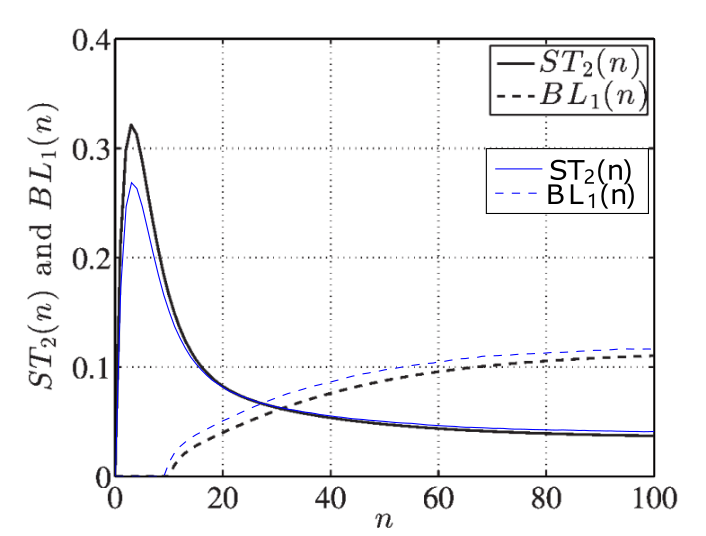
\includegraphics[width=0.5\linewidth]{2_c.png}
	\caption{Performance contrast of a two-machine geometric line $ST_2(n) \ and\ BL_2(n)$}
	\label{2_c}
\end{figure*}

\begin{figure*}[!h]
	\centering
	\subfigure[]{
		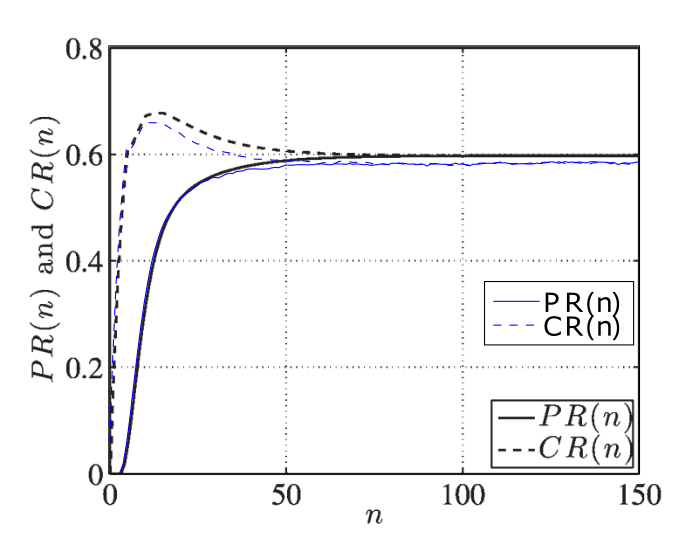
\includegraphics[width=0.45\linewidth,height=0.35\linewidth]{4_a.png}
		\label{d four machine pr and cr}}
	\subfigure[]{
		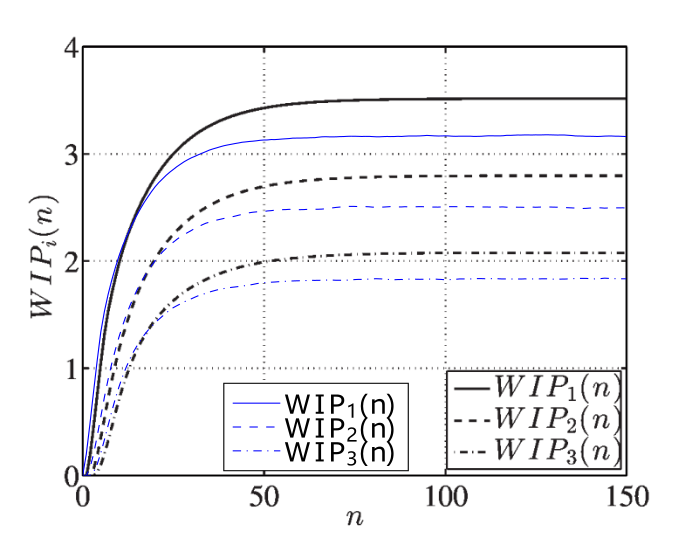
\includegraphics[width=0.45\linewidth,height=0.35\linewidth]{4_b.png}	
		 \label{d four machine wip}}
	\subfigure[]{
		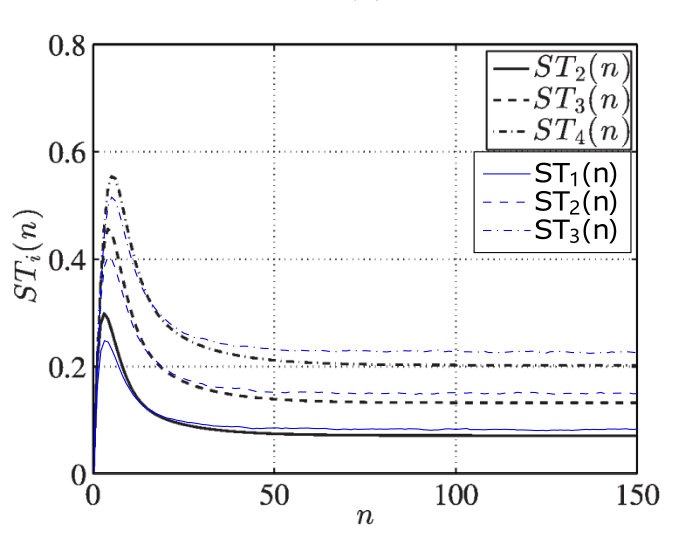
\includegraphics[width=0.45\linewidth,height=0.35\linewidth]{4_c.png}	
		\label{d four machine st}}
	\subfigure[]{
		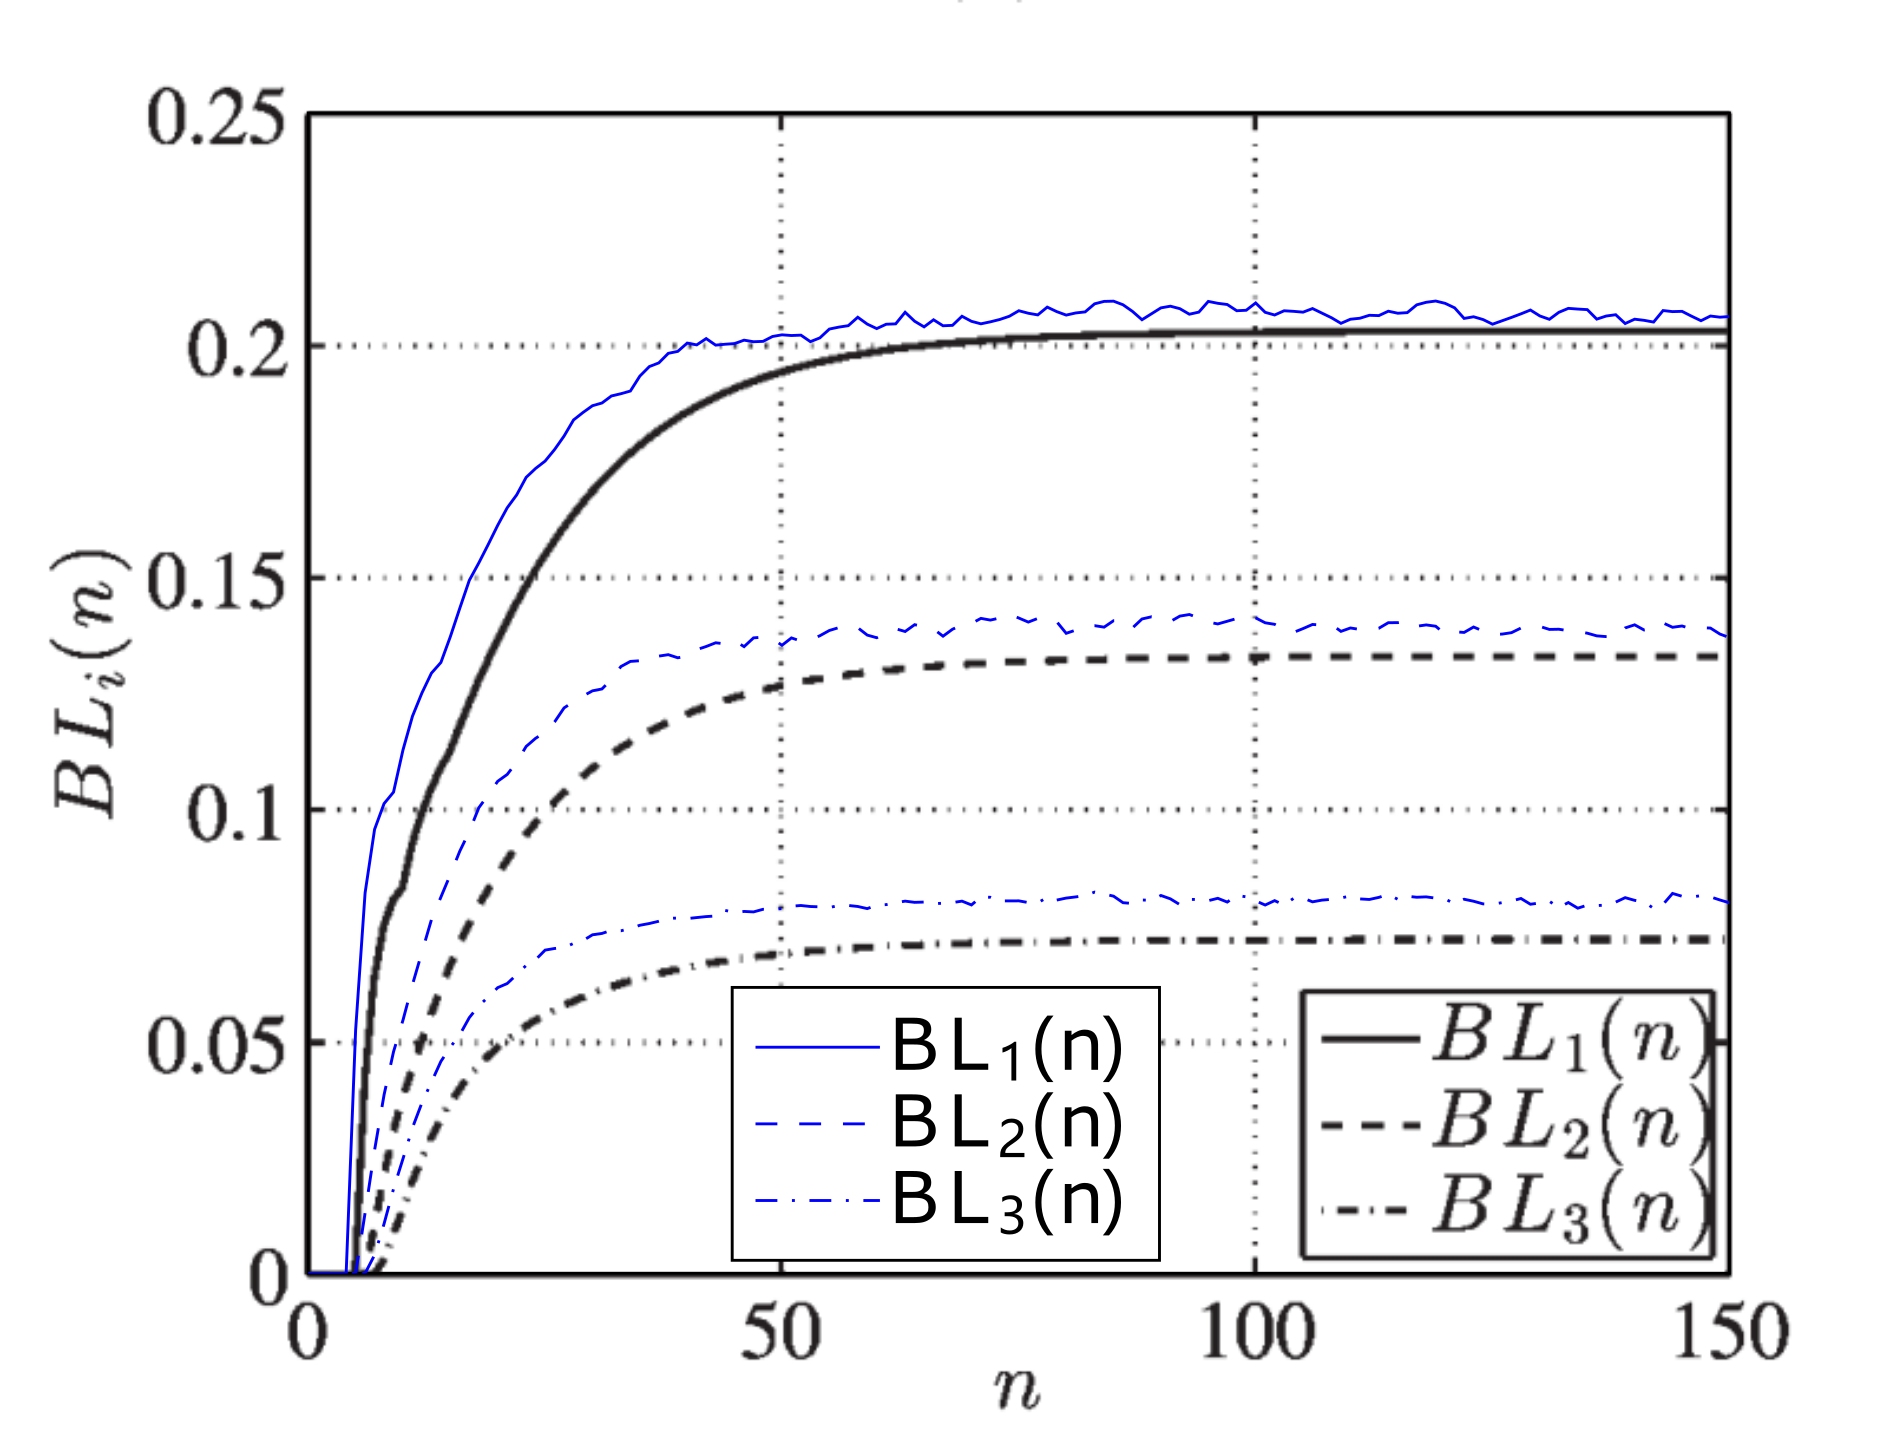
\includegraphics[width=0.45\linewidth,height=0.35\linewidth]{4_d.png}	
		\label{d four machine bl}}
	\caption{Transients of a four-machine geometric line. (a) $PR(n) \ and\ CR(n)$;(b) $WIP(n)$; (c) $ST_i(n)$;(d) $BL_i(n)$.}
	\label{differece four}
\end{figure*}

For the reasons of these difference, we suppose a few points: First, we doubt that whether the lack of enough quantity of samples cause the problem. But when we enlarege the quantity of simulation time from 10000 to 100000, we found no apparent difference from the result. Second, due to that we don't know what kind of programming language the reseachers coding with, a probable cause may be we take a different platform to programm with, and that may cause some accuracy problem. Third, we also doubt that the researchers may do some kind of curve smoothing in oder to present a perfect result.
% \chapter{Impact Analysis in Variation of the Buffer Size}
\label{D_Kapitel}
\noindent In this chapter we attepmt to explorer the relationship between the  paramters and the transient performance of a multi-machine line with five machines. 

\begin{figure*}[!h]
    \centering
		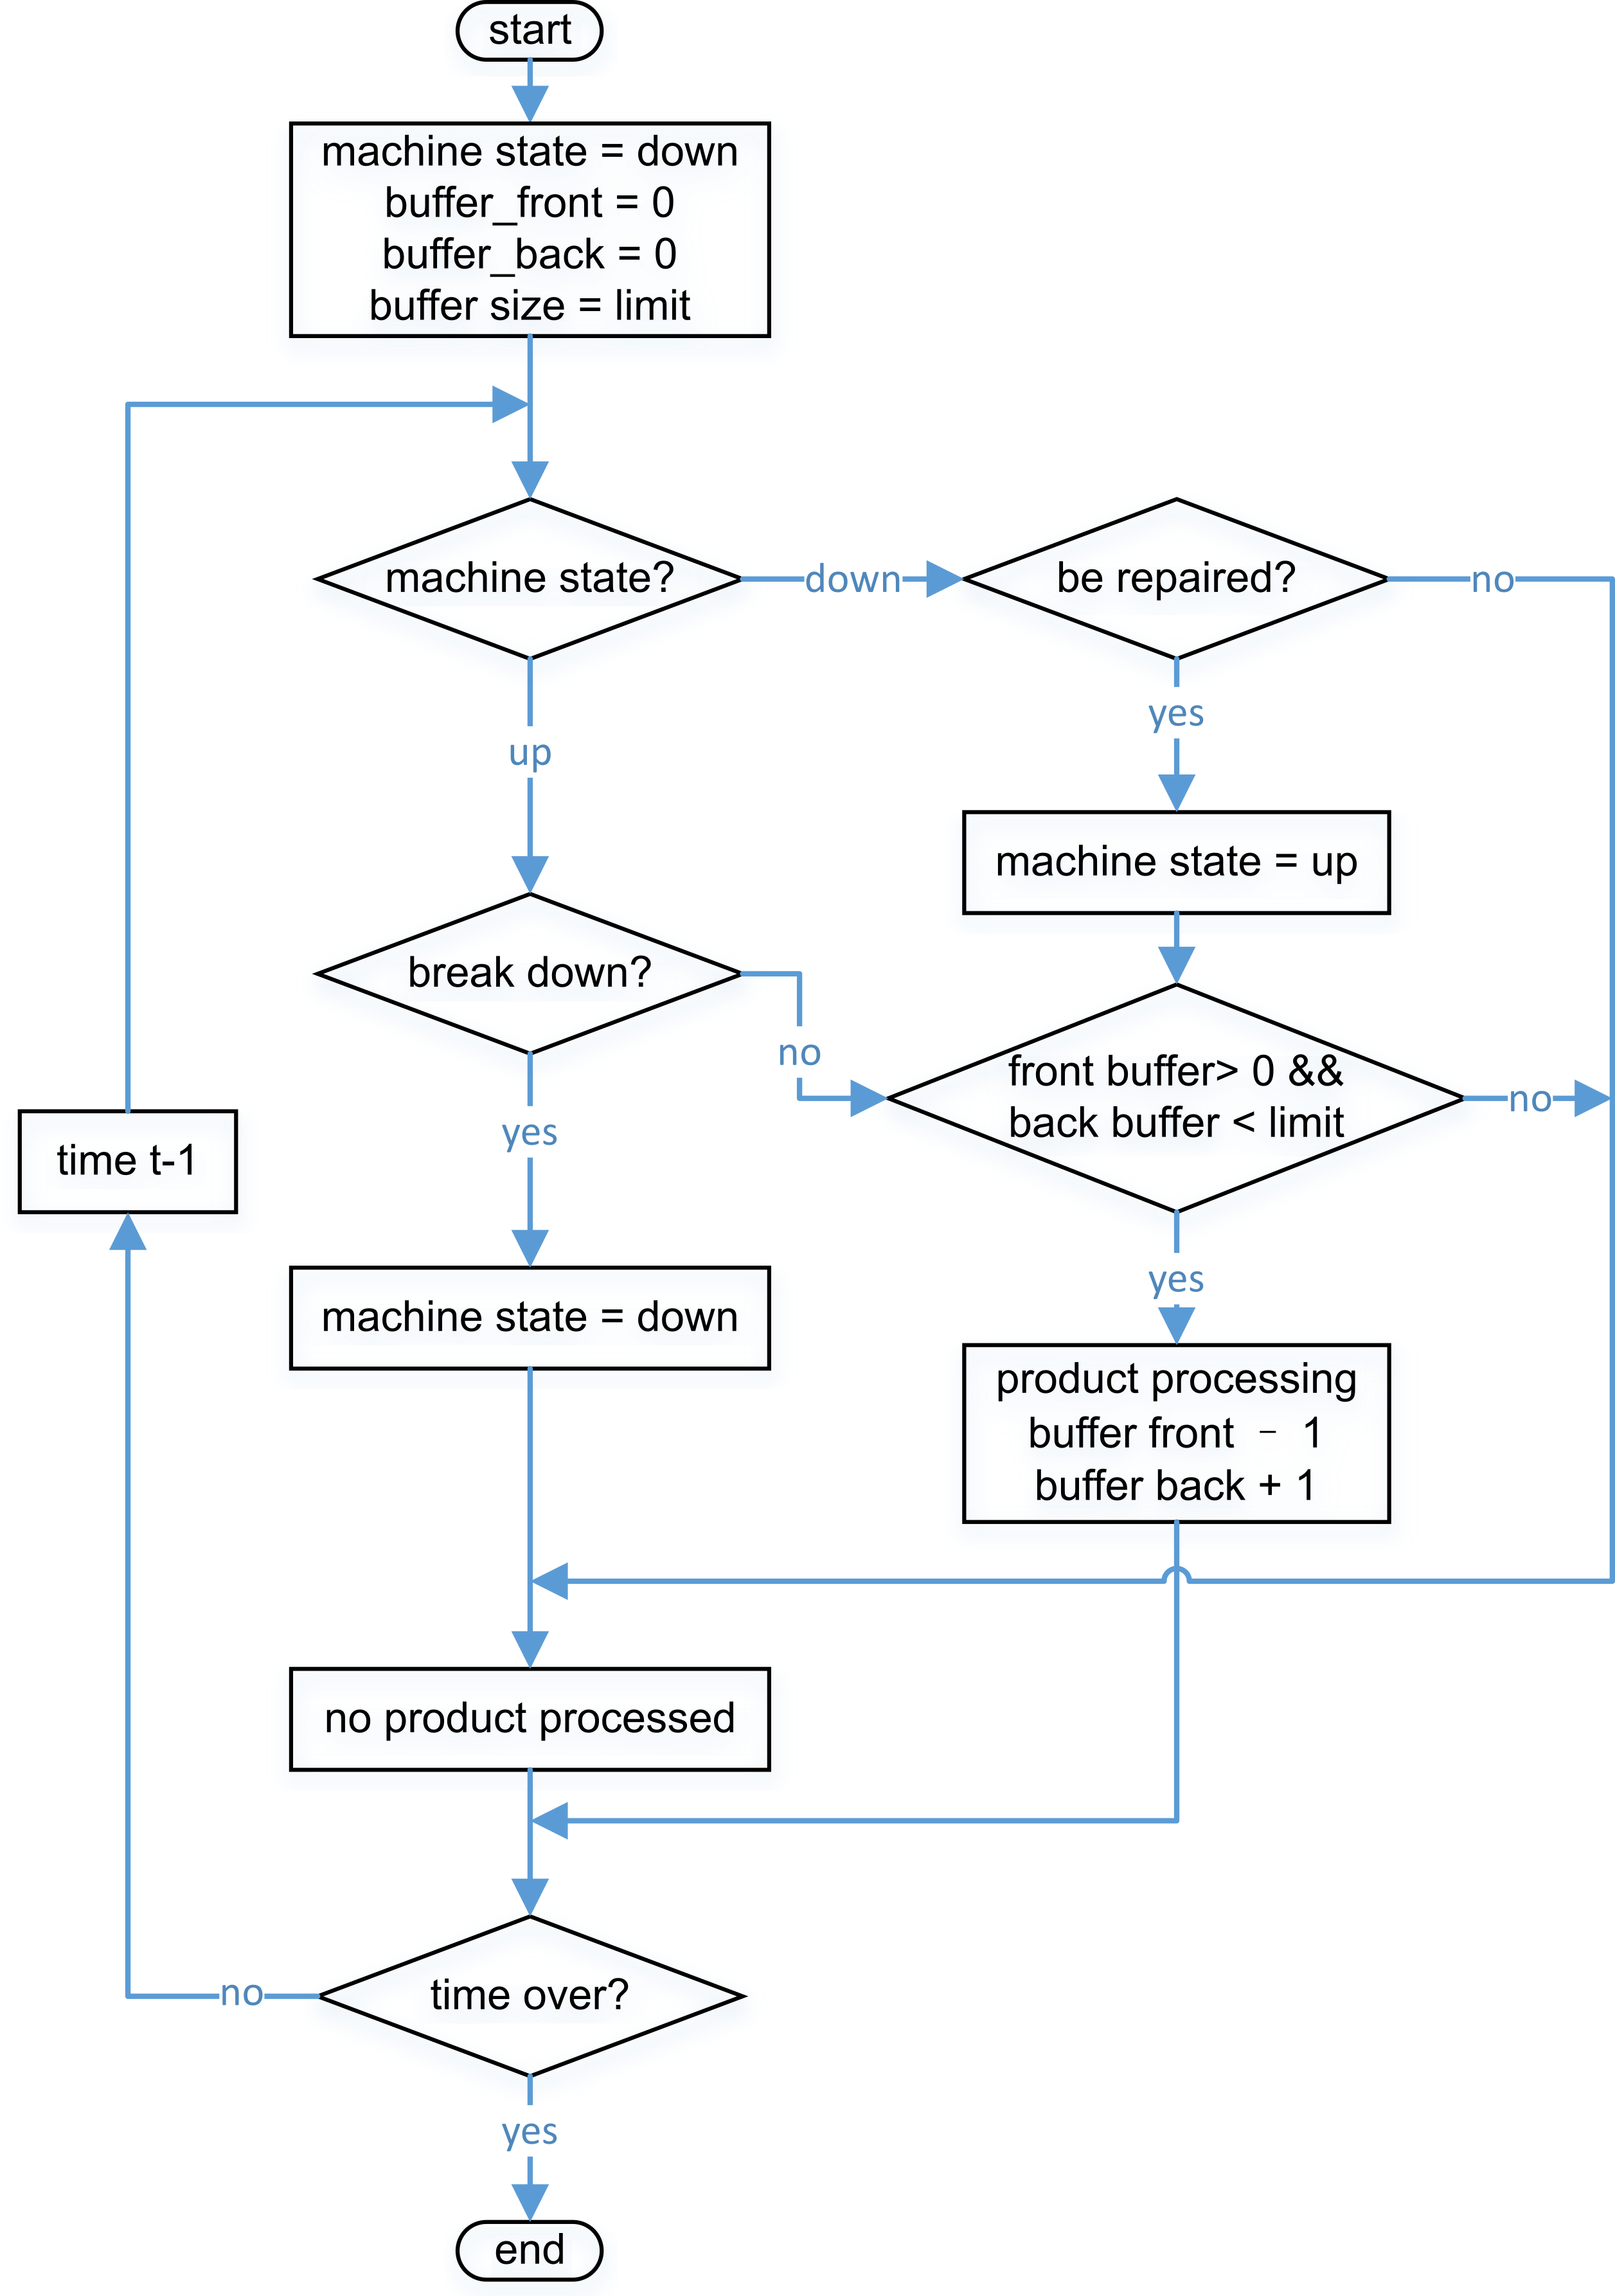
\includegraphics[width=0.62\linewidth]{procedure.png}	
	\caption{Flow chart of Procedure.}
    \label{flow chart}
\end{figure*}
\section{Procedure Description}
\noindent We suppose that a suitable buffer size can help to improve the transient performance of the production line. On the other hand, if the buffer size is designed . Therefore, we design a experiment on a five-machine production-line model. We use the following parameters:
\begin{displaymath}
    P = 0.05, R = 0.2, N = 1,...20, \text{All Buffer storage = epmty}
\end{displaymath}

In order to describe the procedure, we use a flow chart to illustrate the critical part of the program logic. At the beginning, we initialize all the parameters given in the file ''simulation.py''. Next, the parameters are passed to the file called ''multi\_machine.py'', and a certain amount of this object are created from the \pythoninline{class MultiMachine} to calculate the average of the cirtical values. Furthermore, the related machine objects and buffer objects will be created and simulated according to the procedure shown in flow chart. 

When the programm creates a simulated geomatric machine line, it first initiallize states of all machines and storages of all buffers. After that, in each time slot two conditional function will be called sequentially in order to make sure whether the machine break down , and if it can to be repaired or may break down according to its present state espectively. If the machine is in good condition (i.e. it can work), thereupon another conditional function will be called to test if the buffer in front of the machine has at least one product (except the first machine) or the buffer at the end of the machine has enough space to receive one new product (except the last machine). If all these conditions filling, then the machine produce a product, and at the same time take one product from the front buffer with put a product in the back buffer.

\section{Results and Discussion}
\noindent After the simulation, we collected the data of evaluation of transient performance of the geomatric machine lines. The Figure 1 shows with the buffer size enlarging the trend of the production rate. Figure 2 shows that this trend of 

\begin{figure*}[!h]
    \centering
    \subfigure[]{                
		\includegraphics[width=0.45\linewidth]{pr_n.tikz}	
    % \caption{Variance of Production Rate with N buffer size.}
    \label{pr buffer size}
    }
    \subfigure[]{
        \includegraphics[width=0.45\linewidth]{cr_n.tikz}
        % \caption{Variance of Consumption Rate with N buffer size.}
    \label{cr buffer size}
        }
    \caption{Variance of Transient Parameters. (a) Production Rate; (b) Consumption Rate.}
    \label{p c rate N buffer}
\end{figure*}
% \chapter{Conclusion}
\label{E_Kapitel}
\noindent Nowadays, improving productivity and quality has becoming a core concern in manufacturing research. With global energy crisis and environmental problems, reducing energy costs and waste gas emission has been a significant issue for the manufacturing industry. In order to solve these problems, researchers investigate a lot of effort in the study of production systems. 

Obviously, in comparison to the enrmous studies on steady state performance of production lines \cite{gershwin1991assembly,liu1990approximate}, very few results have been made in literature on the transient behavior of production systems. The goal of this research is to use the python to implement the simulations of the geometric machine model, and optimize the buffer size of a five-machine production lines.

In this paper, we studied the transient performance evaluation of serial production lines with machines with geometric reliability model and finite buffers. The contribution are givne in this work as follows:

\begin{itemize}
    \item First part we review the research works of production systems, then make a summary, i.e. the past works in this field most focused on the steady performance of the production lines, while the transient evaluation still need more effort to be devoted. The detailed derivations of the model are given in Chapter 2.
    \item Next, we make a brief introduction of the theory basis. In addition, the assumptions of the model of serial produciton line systems are presented and the performance measures are defined. The implementation of the system models are give in next chapter.
    \item In Chapter 3, we use the python to implement three models, the single-machine production lines, two-machine with a buffer, and multi-machine with buffers. And we separately give the performance measures according to each kind of production lines. On the other hand, we make a comparison of the results with another work, and attempt to analyse the difference of the results. 
    \item Moreover, in the next chapter we also make a study about the impact of buffer sizes on transient performace. In order to find the most suitable buffer size, we designed a procedure to analyse the critical transient performance. Eventual, it come to a conclusion that for a five-machine serial production lines 10 buffer is a more balanced size for each buffer.  
    
\end{itemize}

It is plausible that still some limitations may exist in the results obtained.
Firstly, the computational costs are still very large especially when the parameter changes and more production line devoted to calculate the mathematical expectation. In addition, the bottleneck of the prodution lines may still be dedicated efforts to investigate , and continuous improvement can be studied. Furthermore, the the structure of the model may be still simplified. Assembly systems and other production with complex structures remains to be explore. 

% % #######################################################################
% Anhang
% #######################################################################

\begin{appendix}

% #######################################################################
\chapter{Source Code of all models}

The followings are the python source code according to different models

The Individual machine model

File ''individual.py''
\pythonexternal{pycodes/individual/individual.py}

File ''simu1.py''
\pythonexternal{pycodes/individual/simu1.py}

The Two-machine model

File ''individual.py''
\pythonexternal{pycodes/Two_machine/individual.py}

File ''buffer.py''
\pythonexternal{pycodes/Two_machine/buffer.py}

File ''twomachine.py''
\pythonexternal{pycodes/Two_machine/twomachine.py}

File ''sim2.py''
\pythonexternal{pycodes/Two_machine/sim2.py}

The Multi-machine model

File ''individual.py''
\pythonexternal{pycodes/Multi/individual.py}

File ''buffer.py''
\pythonexternal{pycodes/Multi/buffer.py}

File ''multimachine.py''
\pythonexternal{pycodes/Multi/multimachine.py}

File ''sim4.py''
\pythonexternal{pycodes/Multi/sim4.py}

The study in Chapter 4 

File ''individual.py'' is same as file ''individual.py'' in Multi-machine model

File ''buffer.py'' is same as file ''buffer.py'' in Multi-machine model

File ''multimachine.py'' is same as file ''multimachine.py'' in Multi-machine model

File ''simulation.py''
\pythonexternal{pycodes/Procedure1/simulation.py}
\end{appendix}
% \input{part/part7}

% #######################################################################
% Abbildungsverzeichnis
% #######################################################################

% \addcontentsline{toc}{chapter}{Abbildungsverzeichnis} \listoffigures

% #######################################################################
% Tabellenverzeichnis
% #######################################################################

%\newpage
%\addcontentsline{toc}{chapter}{Tabellenverzeichnis} \listoftables

% #######################################################################
% Literaturverzeichnis
% #######################################################################

%\clearpage
\newpage
\renewcommand{\bibname}{List of References}
\pagestyle{fancy}
\lhead{\textsl{List of References}}
\rhead{\thepage}
\cfoot{}
\bibliographystyle{unsrtdin}
\bibliography{./LiteraturVorlage}
\addcontentsline{toc}{chapter}{\bibname}

\end{document}
